\section{Introduction}
\label{sec:introduction}

Globally, it is estimated that people spend approximately 90\% of their time indoors \cite{schweizer_indoor_2007, klepeis_national_2001} and breathe 11.000 liters of air per day \cite{corlan_importance_2021}. Suboptimal indoor air quality (IAQ) conditions affect building occupants' experiences of comfort and insufficient ventilation in indoor environments is proven to play significant roles in occupants' well-being, health, and cognitive functions \cite{, wang_how_2021, kim_analyzing_2019}. 

The perceived comfort of occupants is influenced by the overall Indoor Environmental Quality (IEQ) consisting of several key metrics (e.g. mechanical ventilation, temperature regulation, natural lighting) to create a combined IEQ index for a specific indoor space \cite{kulshreshtha_indoor_2024}. Among these metrics, indoor air quality stands out as a crucial factor deserving special attention due to its invisibility to occupants \cite{son_perceived_2023}, polluted air goes undetected by smell or sight, underscoring the importance of monitoring and maintaining optimal indoor air quality.

Furthermore, mechanical ventilation systems in buildings operate discreetly and are frequently insufficient for ventilation in densely populated small rooms like meeting rooms, laboratory offices, or hot-desking work areas \cite{silva_post-occupancy_2017}, which contributes to occupants' perceived lack of control. Since these systems are typically automated \cite{persily_challenges_2015} and cannot be directly regulated or controlled by occupants themselves \cite{kim_automatic_2019}. 

This creates an interplay between occupants' effects on comfort, built environments, and computing technologies (see \hyperref[fig:complexity]{Figure \ref*{fig:complexity}}) researched in an overarching interdisciplinary field of study, known as Human-Building Interaction (HBI) \cite{alavi_introduction_2019}. This research specifically focuses on understanding occupants' needs through in-the-wild \cite{rogers_moving_2017} studies gaining insight into occupants' awareness, collecting indoor air quality data in designated spaces, prototyping data physicalization devices to visualize indoor air quality, and using these designs as data probing tool \cite{zimmerman_research_2007} evaluating their effectiveness with the overarching objective of obtaining insights into occupants' comfort levels and facilitating their adoption of preventive measures against poor indoor air quality \cite{zhong_complexity_2021}. 

While research on defining comfort within indoor buildings \cite{alavi_comfort_2017}, gathering and analyzing sensory air quality data \cite{corlan_importance_2021}, and the effects of poor air quality are prevalent \cite{klepeis_national_2001}, there remains a research gap in understanding occupants' behavior and their subjective needs, along with limited research on how design solutions that visualize environmental data and computing installations can empower occupants, particularly within the field of physically visualizing data to convey IAQ to building occupants in real-time. 

\begin{figure}[h]
    \centering
    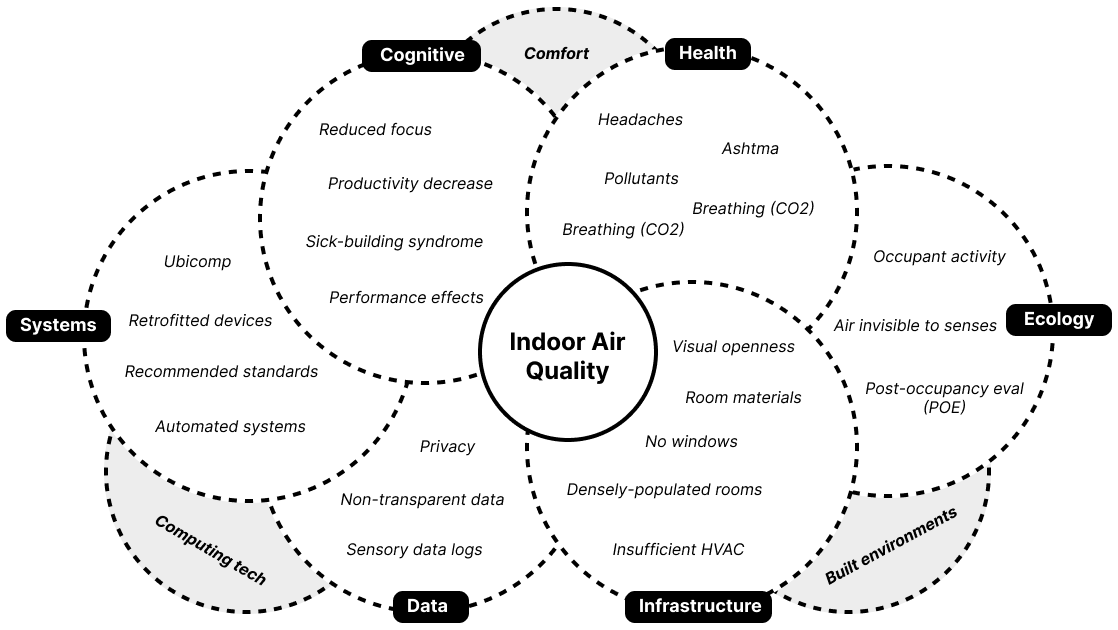
\includegraphics[width=0.5\textwidth]{complexity_diagram_indoor_air_quality.png}
    \caption{Complexity diagram providing an overview of the effects of IAQ and needs of occupants \cite{schweizer_indoor_2007, wang_how_2021, kim_analyzing_2019, alavi_comfort_2017, corlan_importance_2021, klepeis_national_2001}}
    \label{fig:complexity}
\end{figure}


\subsection{Research questions}

In order to research intervention strategies for improving indoor air quality, the following main research question is formulated: \\

\emph{RQ: How can real-time sensory measurements and future predictions of air quality be physically visualised in specific indoor spaces integrating both environmental information and elements that increase awareness among occupants facilitating their adoption of preventive measures against poor air quality?}\label{rq:1} \\

To effectively answer this main research question, this research is guided by the following supporting sub-questions ("sq" for "subquestion") that also serve as objectives to delineate the necessary knowledge: \\


\begin{enumerate}
    \renewcommand{\labelenumi}{SQ\arabic{enumi}:}
    \item \emph{How can environmental information related to air quality, such as pollutant concentrations and ventilation rates, be incorporated into the visual representations?}\label{subq:1}
    \item \emph{How do different types of physical visualizations impact occupants' understanding of air quality and their willingness to adopt preventive measures?}\label{subq:2}
    \item \emph{How do occupants' perceptions and behaviors regarding indoor air quality change over time, from pre to post-installation of the physical representation of poor air quality?}\label{subq:3}\\
\end{enumerate}